\begin{frame}
	\frametitle{Slides and Examples}

        \begin{itemize}
		\item Slides:\\
                  \url{https://depot.tu-dortmund.de/dlep3}
		\item Examples:\\ 
                  \url{https://depot.tu-dortmund.de/5al36} 
        \end{itemize}

\end{frame}

\begin{frame}
  \frametitle{About CMake}

      \begin{block}{CMake Features}
        \begin{itemize}
          \item Open-source application for 'managing the build process' of a software package
          \item CMake is available on all major platforms (Linux, Windows, MacOS, ...) 
          \item Supports source directory trees that depend on multiple libraries
          \item CMake is a script language that includes almost all basic programming language elements
          \item CMake generates a native build environment for the OS it is executed on
          \item Supports in-place and out-of-place builds
          \item Can generate project files for various IDEs (Visual Studio, Xcode, Eclipse, ...)
          \item Has a mechanism to locate libraries in the OS
          \item Can download missing libraries on demand
        \end{itemize}
      \end{block}

\end{frame}


\begin{frame}
  \frametitle{ParaView Software Ecosystem}
  \vspace{-0.9cm}
  \begin{tikzpicture}[remember picture,overlay]
    \tikzset{shift={(current page.center)},yshift=-1.5cm}

    \node[text width=8cm] (C1) at (-8, -0.0) {
      \begin{block}{VTK}
        \begin{itemize}
          \item Visualization backend
          \item Uses OpenGL
        \end{itemize}
      \end{block}
    };

    \node[text width=8cm] (C2) at (8,-0.7) {
      \begin{block}{Qt (cute)}
        \begin{itemize}
          \item Provides widges and other GUI controls
          \item Support for modular plugins
        \end{itemize}
      \end{block}
    };

    \node[text width=8cm] (C3) at (0,4) {
      \begin{block}{CMake}
        \begin{itemize}
          \item Script language to control the building process
          \item Generates a wide range of specific build files
        \end{itemize}
      \end{block}
    };

    \node[text width=8cm] (C4) at (0,-4.85) {
      \begin{block}{ParaView}
        \begin{itemize}
          \item VTK visualization by GUI
          \item Scripting via Python
          \item Extension by plugins
        \end{itemize}
      \end{block}
    };

\end{tikzpicture}
\end{frame}


\begin{frame}
  \frametitle{Use Cases of Visualization Software}

      \begin{block}{Typical ParaView Use Cases}
        \begin{itemize}
          \item Provide an intuitive illustration of raw simulation data

          \item Highlight key features of specific flow features

          \item Provide an intuitive understanding for non-expert viewers  

          \item Help in the testing/debugging process of CFD software 

          \item Assist during result validation by providing analysis tools  

          \item Convert data in different formats in order to communicate with scientific partners
        \end{itemize}
      \end{block}

\end{frame}

\begin{frame}
  \frametitle{ParaView Interface}

  \begin{tikzpicture}[remember picture,overlay]
    \tikzset{shift={(current page.center)},yshift=-1.5cm}

    \node[align=center,scale=0.3,transform shape] (C1) at (0,0)
    {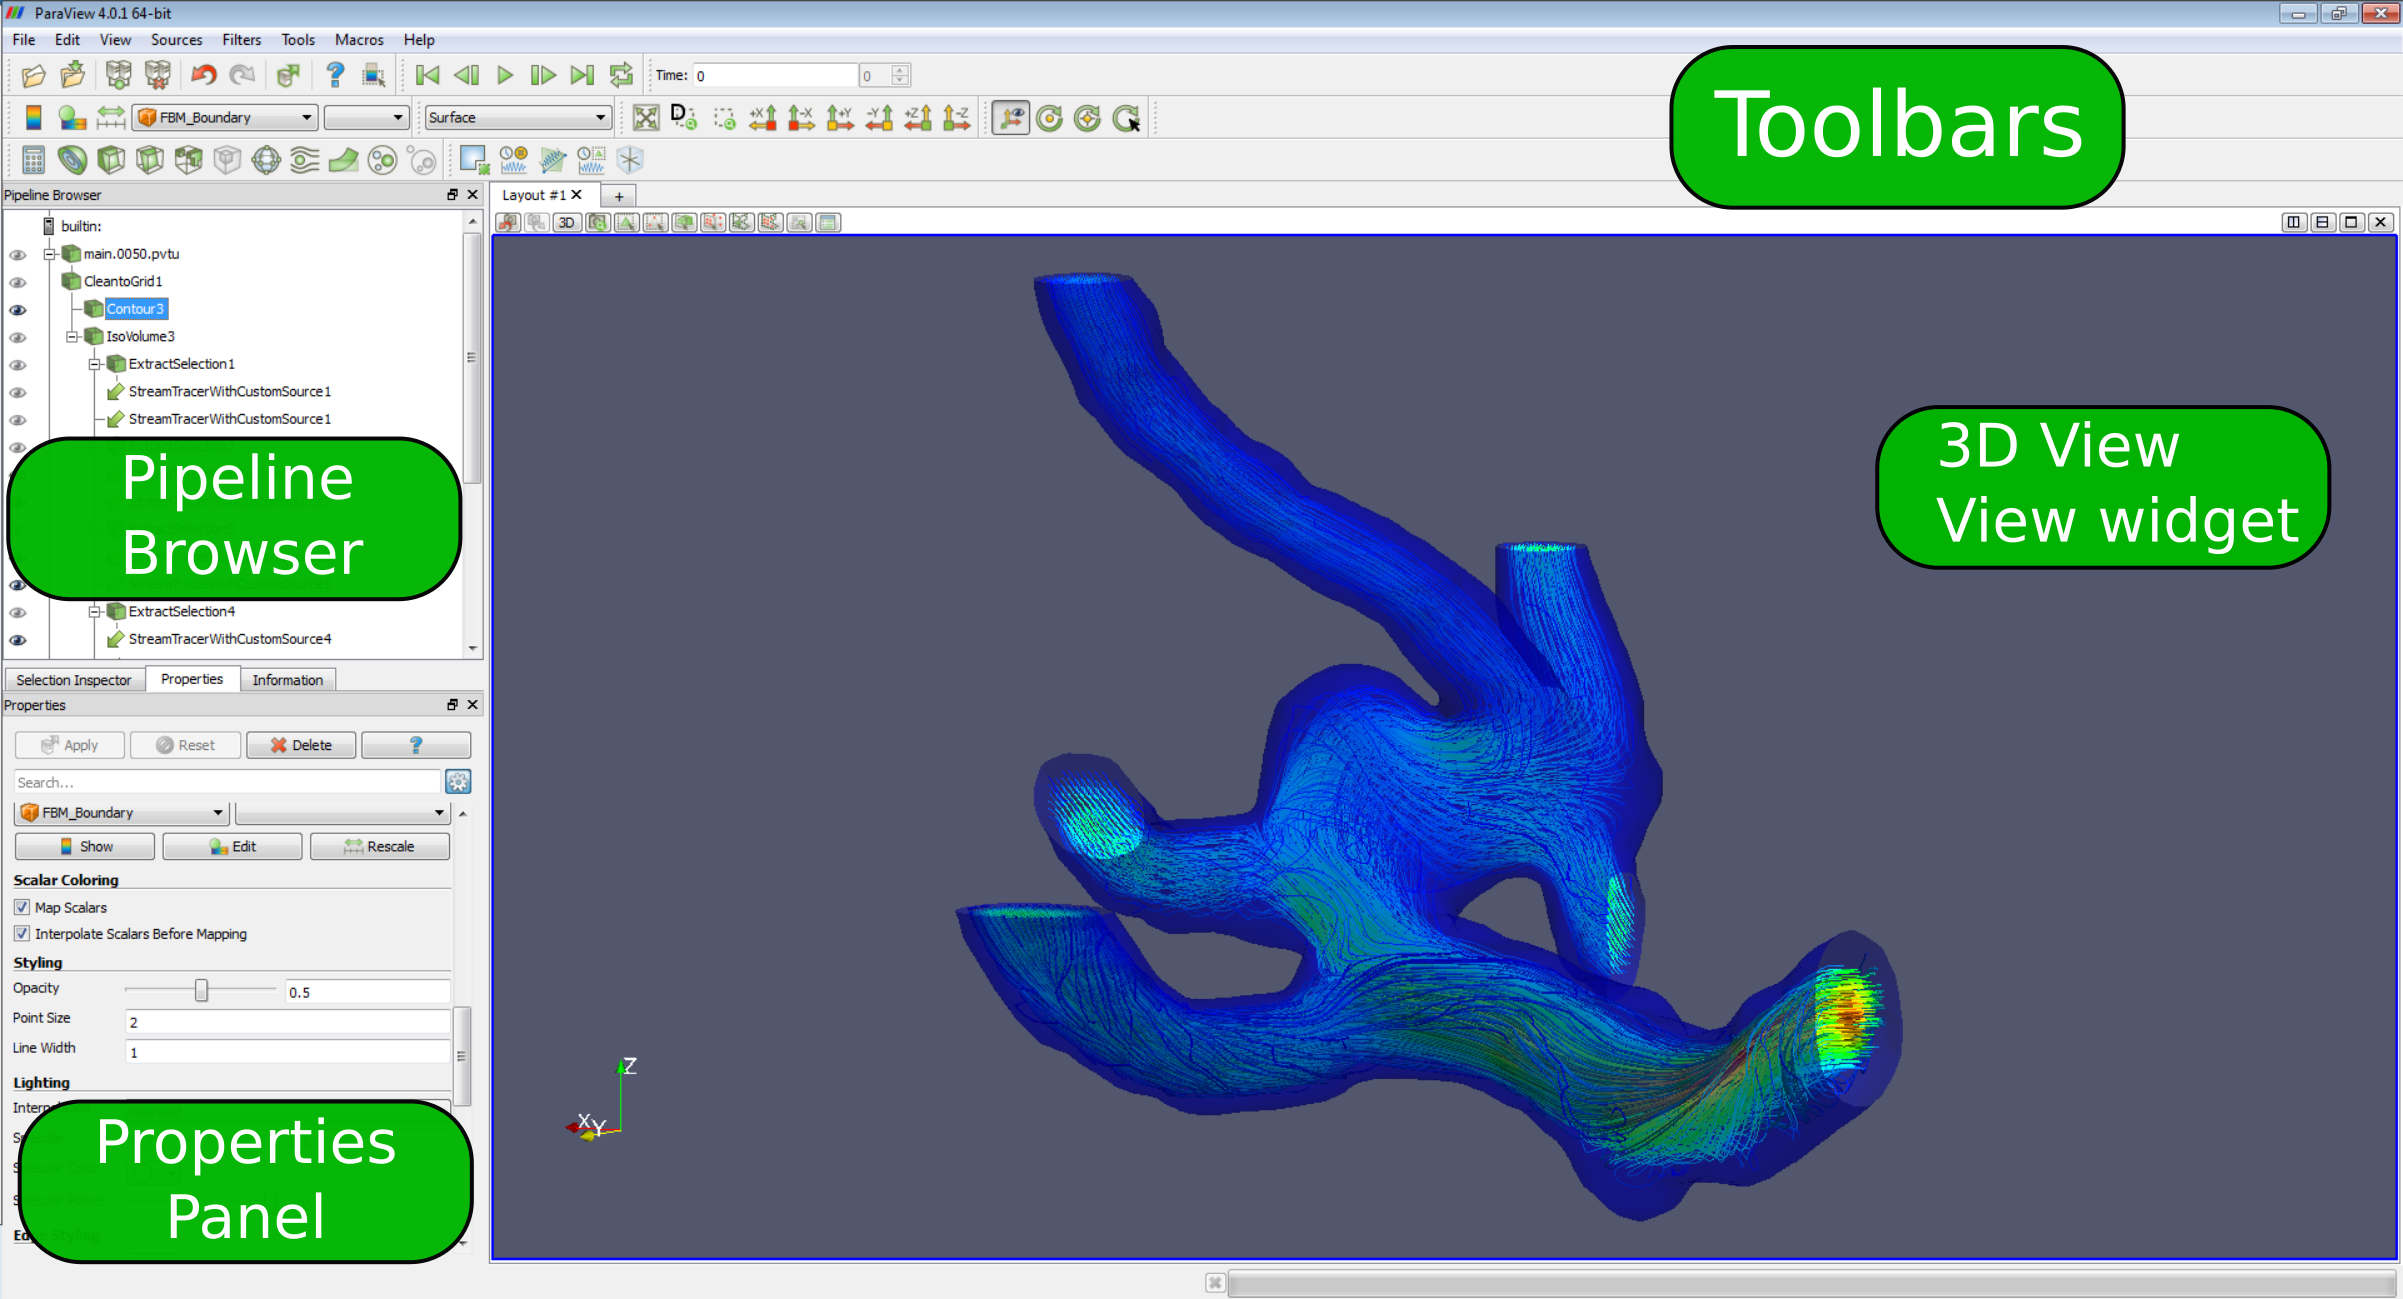
\includegraphics{screenshots/pv-gui.png}};

\end{tikzpicture}

\end{frame}

\begin{frame}[fragile]
  \frametitle{Filter Pipeline Concept}

    \begin{minipage}{0.45 \textwidth}

      \begin{tikzpicture}%[nodes=draw]

    \node[text width=8cm] (C1) at (-8, 1.25) {
      \begin{block}{Filter Pipeline}
        \begin{itemize}
          \item A \keyword{filter} is an operation on an input data set
          \item Filters can be chained (pipelined)  
          \item More complex visualizations require multiple filters 
        \end{itemize}
      \end{block}
    };

    \node[align=center,scale=0.5,transform shape] (C1) at (-10,-5.0)
    {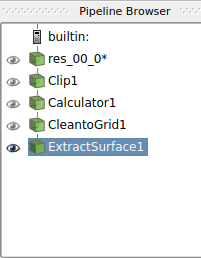
\includegraphics{screenshots/filters.png}};

    \end{tikzpicture}

    \end{minipage}
    \begin{minipage}{0.45 \textwidth}
      \begin{center}
        \begin{tikzpicture}%[nodes=draw]

          \node[align=center,scale=0.189,transform shape] (C1) at (10,-1)
          {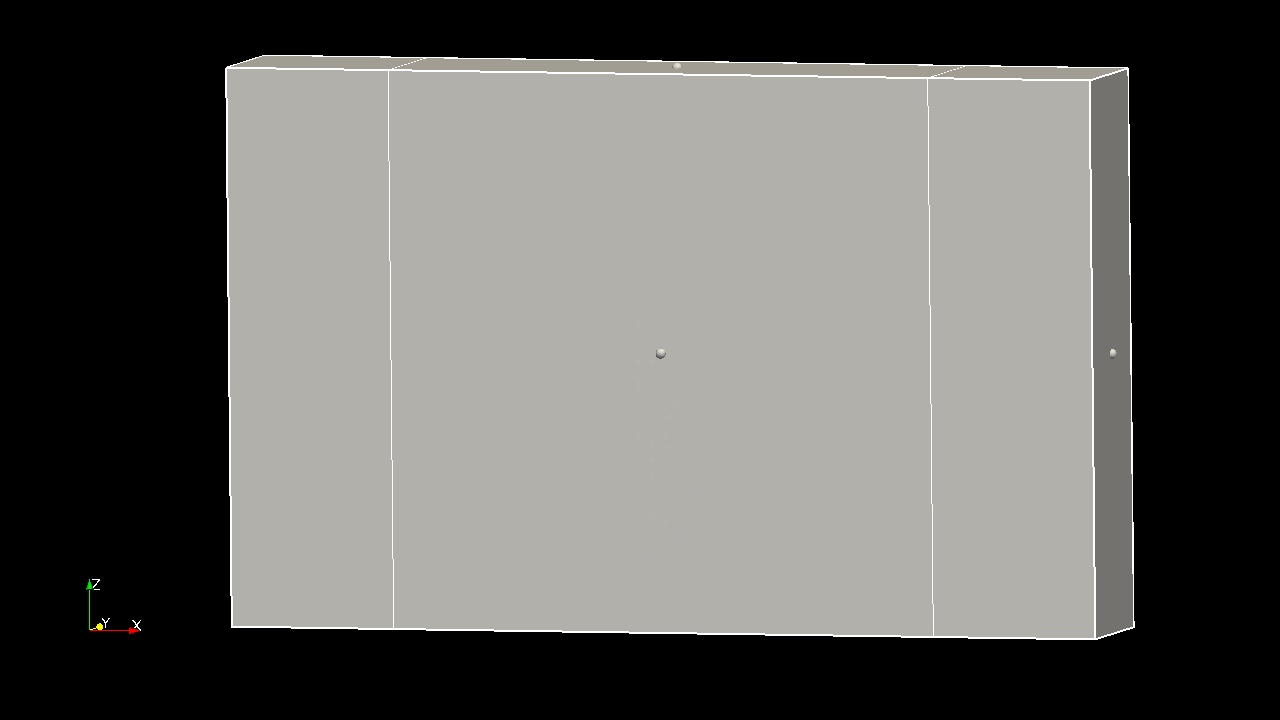
\includegraphics{screenshots/begin-filter.png}};

            \node [scale=2.8,
            fill=TUgreen, 
            single arrow,
            rotate=270, 
            font=\sffamily
            ] at (10.0,-4.22)  
            {\rotatebox{270}{}};

          \node[align=center,scale=0.8,transform shape] (C2) at (10,-8)
          {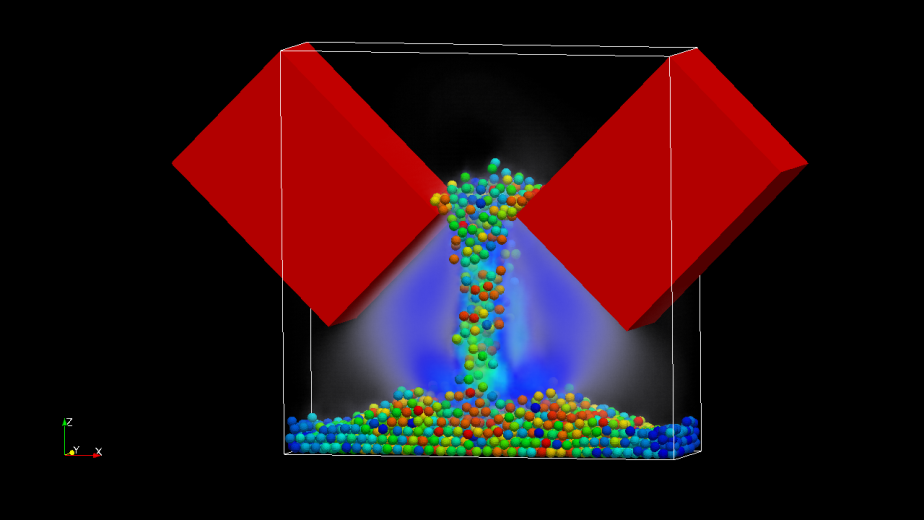
\includegraphics{screenshots/end-filter.png}};

        \end{tikzpicture}
      \end{center}
    \end{minipage}
\end{frame}

\begin{frame}
  \frametitle{Camera and Axes Toolbar}

  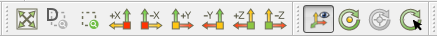
\includegraphics[width=\textwidth]{screenshots/camerabar.png}

    \begin{itemize}
      \item Reset the camera to its default parameters
      \item Magnify a rectangular selection of the view area
      \item Choose a certain coordinate axes plane to look at
      \item Toggle rendering of orientation axes 
      \item Toggle rendering of center of rotation 
      \item Select a new center of rotation 
    \end{itemize}
\end{frame}

\begin{frame}
  \frametitle{Basic Filters}

    \begin{itemize}
      \item \keyword{Slice}: Extract a plane, box-, sphere- or cylinder surface out of a data set
      \item \keyword{Clip}: Extract a plane, box-, sphere- or cylinder volume out of a data set
      \item \keyword{Warp by Scalar}: Visualizes a scalar value by a height extrusion on a 2D data set 
      \item \keyword{Contours}: Increases visibility of different solution contour levels 
      \item \keyword{Surface LIC}: Streamlines on pixel basis, highlights small scale flow features 
      \item \keyword{Glyphs}: Streamlines on pixel basis, highlights small scale flow features 

      \item \keyword{Stream Traces}: Visualizes the pathline of a particle through a \emph{stationary} vector field 
    \end{itemize}

\end{frame}

\begin{frame}
  \frametitle{State Files}

    \begin{itemize}
      \item \keyword{State file}: XML format based file with the ending .pvsm that is used to store the currently applied filters and a reference to the currently loaded data sets to a file
      \item Used to quickly restore a state or to recover from a crash
      \item The reference to the data set can be changed upon loading the state file in order to apply the
        filters to a different data set or if the location of the data on the hard drive has changed
      \item This way state files can be used to exchange a ParaView visualization with collaborators, they only need to set the location of their data set upon loading the state file
      \item State files can be exchanged between different version of ParaView
      \item Accessible from Menu: \keyword{File->Load State...}
    \end{itemize}
        

\end{frame}

\begin{frame}[plain]
  \vspace{3cm}
  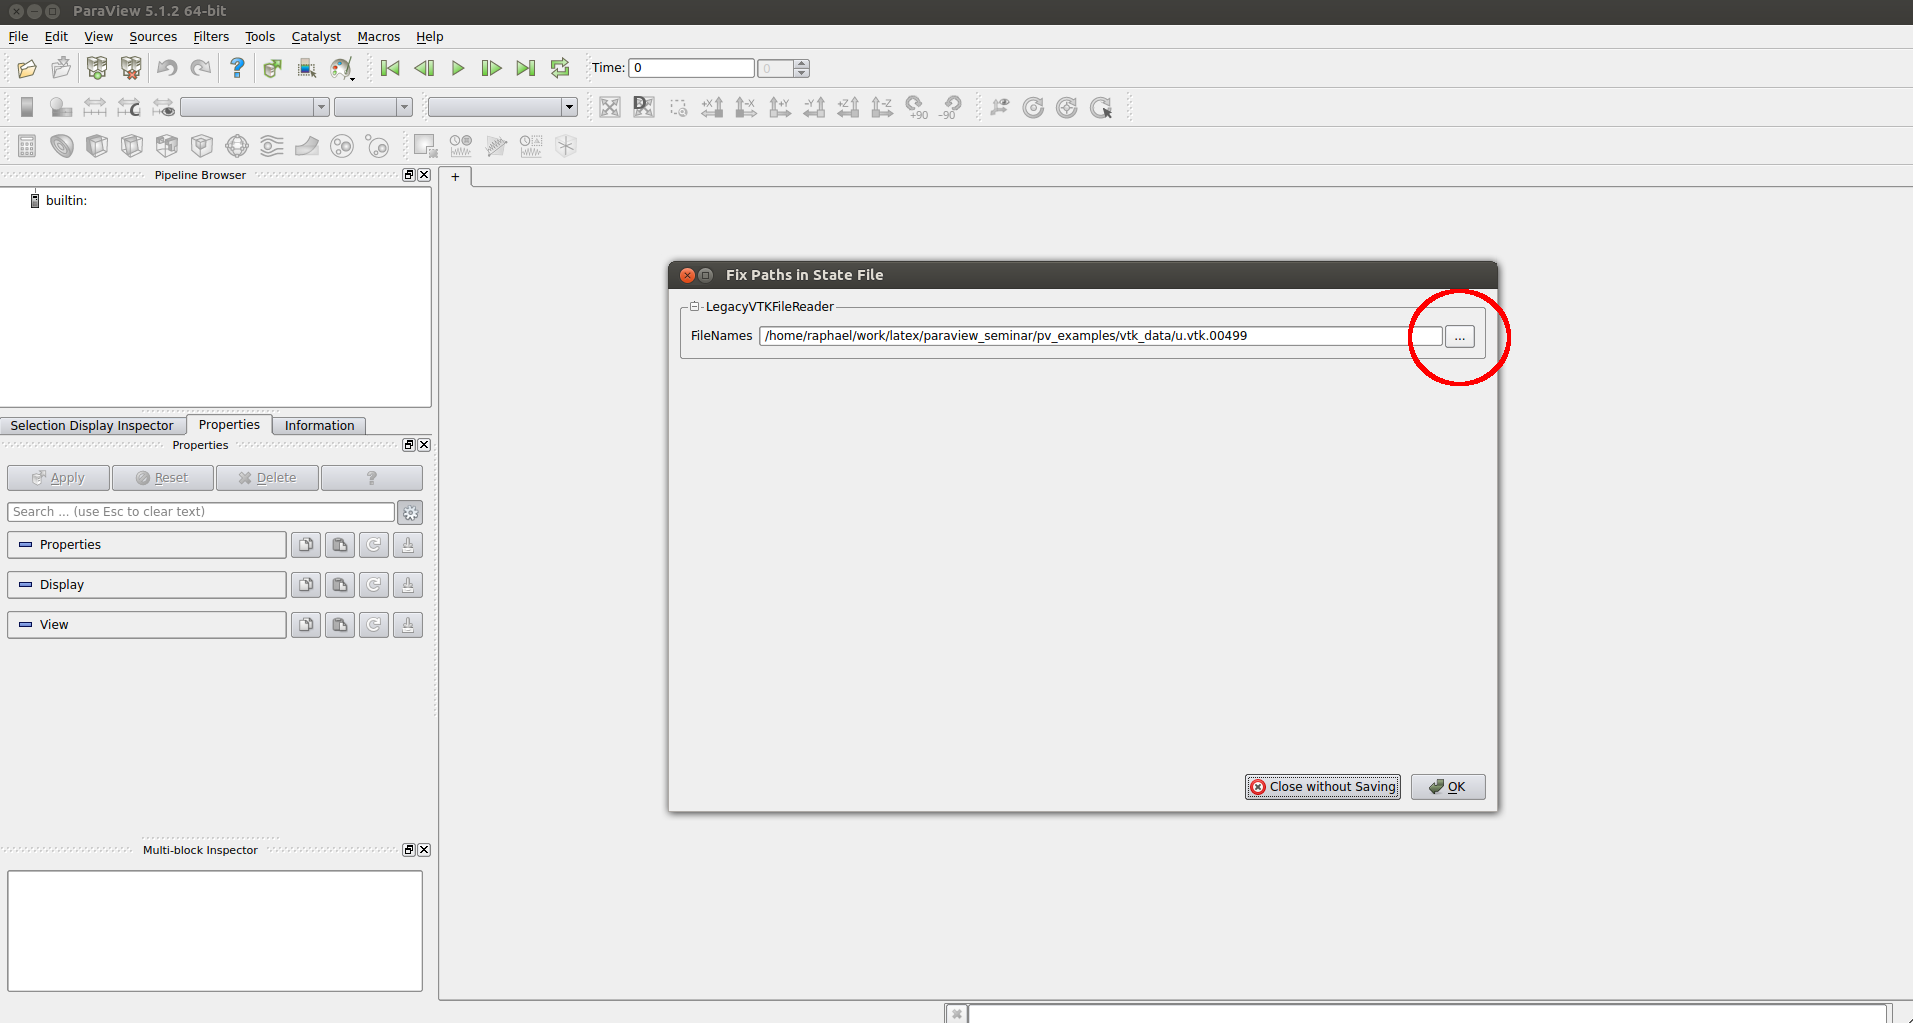
\includegraphics[width=\textwidth]{screenshots/load-state-file.png}
\end{frame}

\begin{frame}
  \frametitle{Examples Files}

    \begin{itemize}
      \item ParaView examples are provided as state files 
      \item Download archive of ParaView examples from:
      \item Extract archive to \kommandozeile{/mypath/to/examples/}
      \kommandozeile{> tar xvfz pv\_examples.tar.gz -C /mypath/to/examples/}
      \item Basic filter examples are located in \kommandozeile{/mypath/to/examples/pv\_examples}
      \item Basic filter examples are located in \kommandozeile{/mypath/to/examples/pv\_examples/BasicFilters}
      \item To load a basic filter example, load the state file and set data path to:
        \kommandozeile{/mypath/to/examples/pv\_examples/vtk\_data/u.vtk}
    \end{itemize}
        

\end{frame}

\begin{frame}
  \frametitle{Basic Filter Gallery I}

    \begin{tikzpicture}%[nodes=draw]

      \node[align=center,scale=0.2,transform shape] (C1) at (0,0)
      {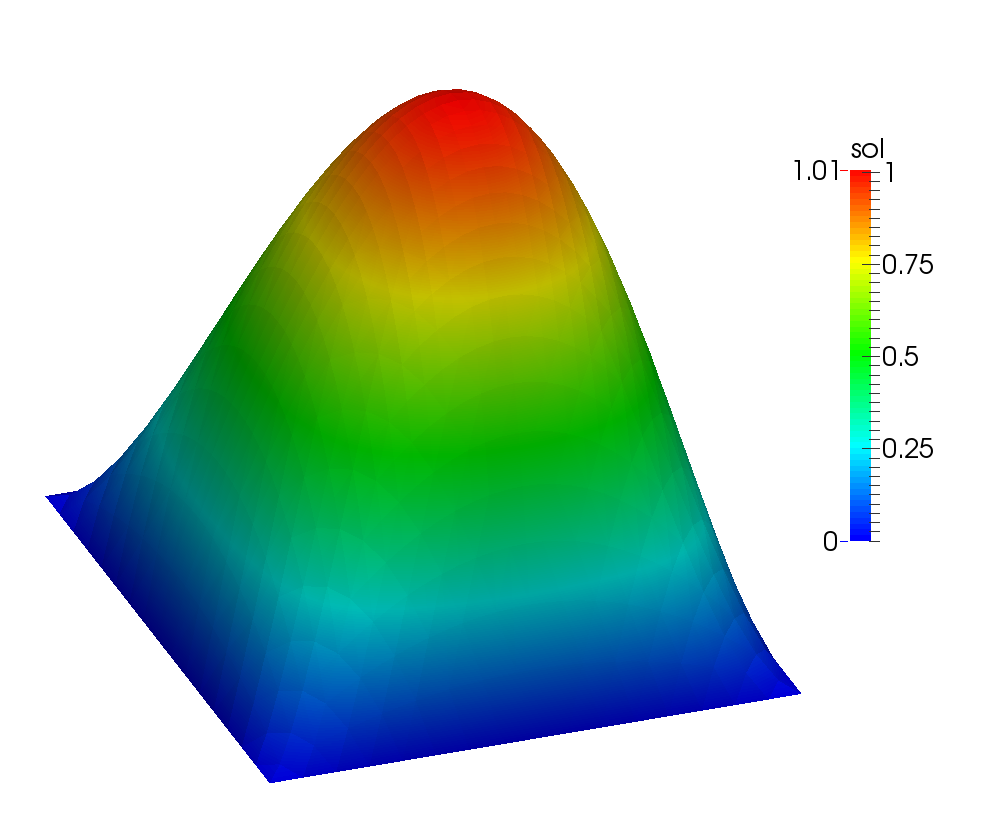
\includegraphics{screenshots/warp-by-scalar.png}};

      \node[align=center,scale=0.2,transform shape] (C2) at (0,-6)
      {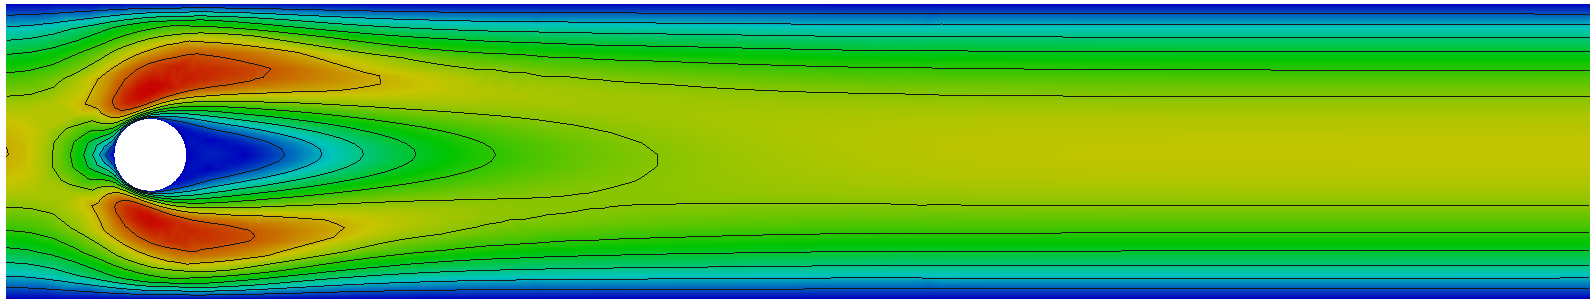
\includegraphics{screenshots/contours.png}};

      \node[align=center,scale=0.2,transform shape] (C3) at (12,-6.05)
      {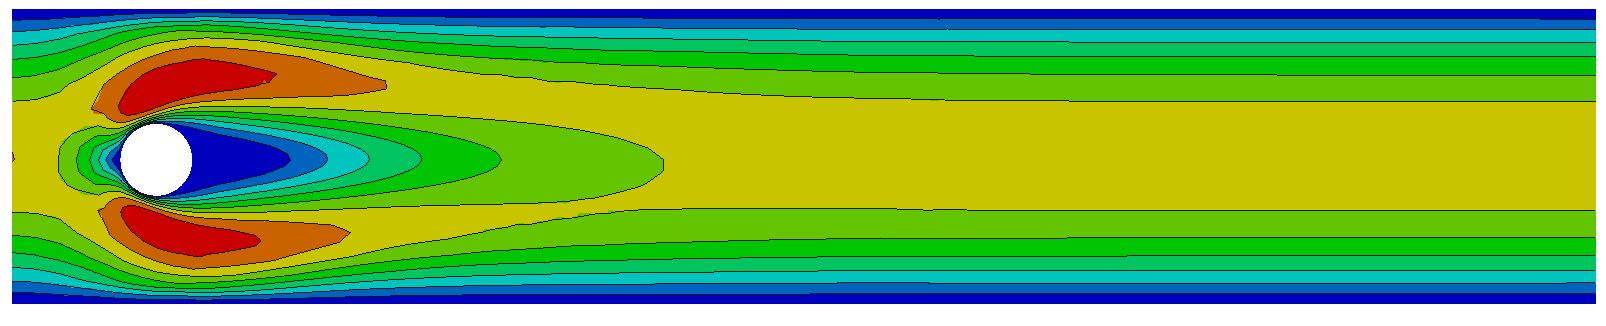
\includegraphics{screenshots/contours_few.png}};

      \node[align=center,scale=0.2,transform shape] (C4) at (12,0)
      {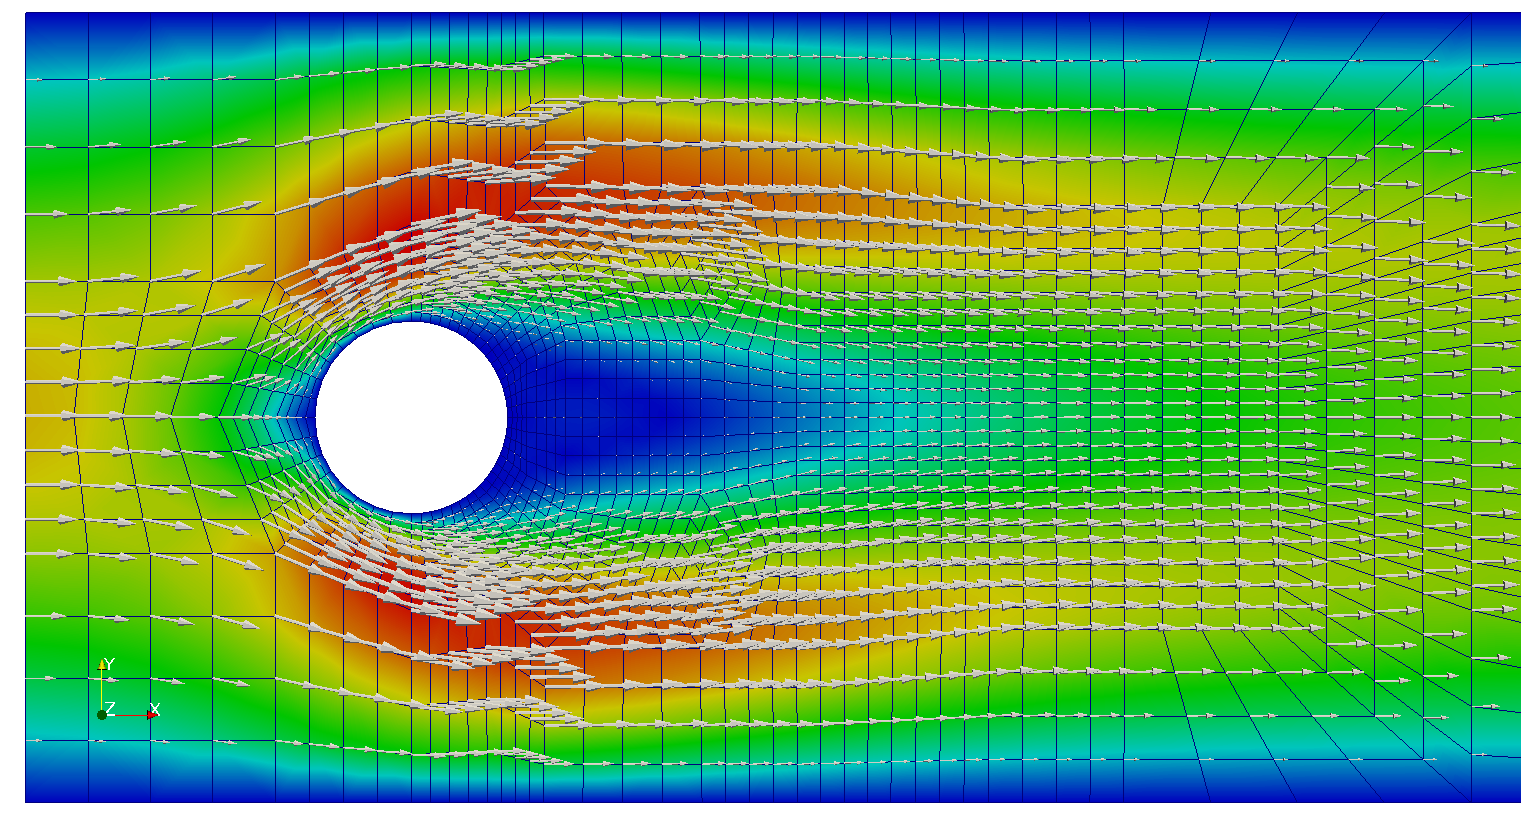
\includegraphics{screenshots/glyphs.png}};

    \end{tikzpicture}

\end{frame}

\begin{frame}

  \frametitle{Basic Filter Gallery II}

    \begin{tikzpicture}%[nodes=draw]

      \node[align=center,scale=0.45,transform shape] (C1) at (0,0)
      {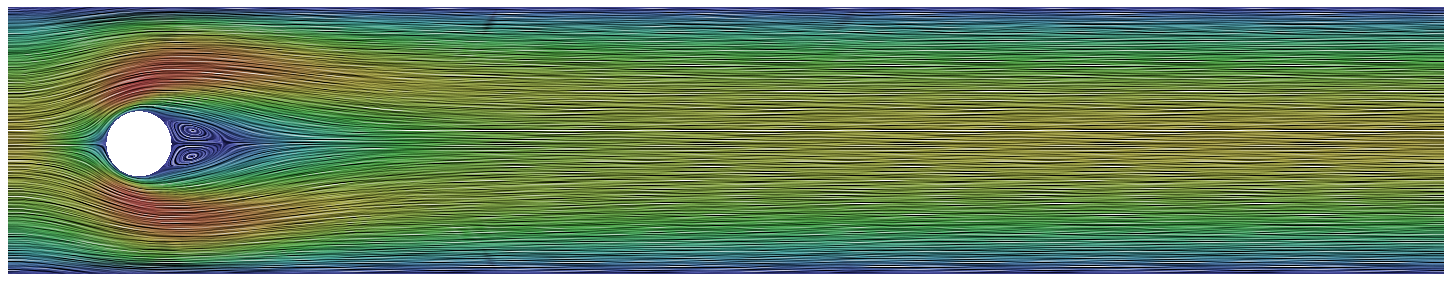
\includegraphics{screenshots/surface_lic_final.png}};

      \node[align=center,scale=0.4,transform shape] (C2) at (0,-6)
      {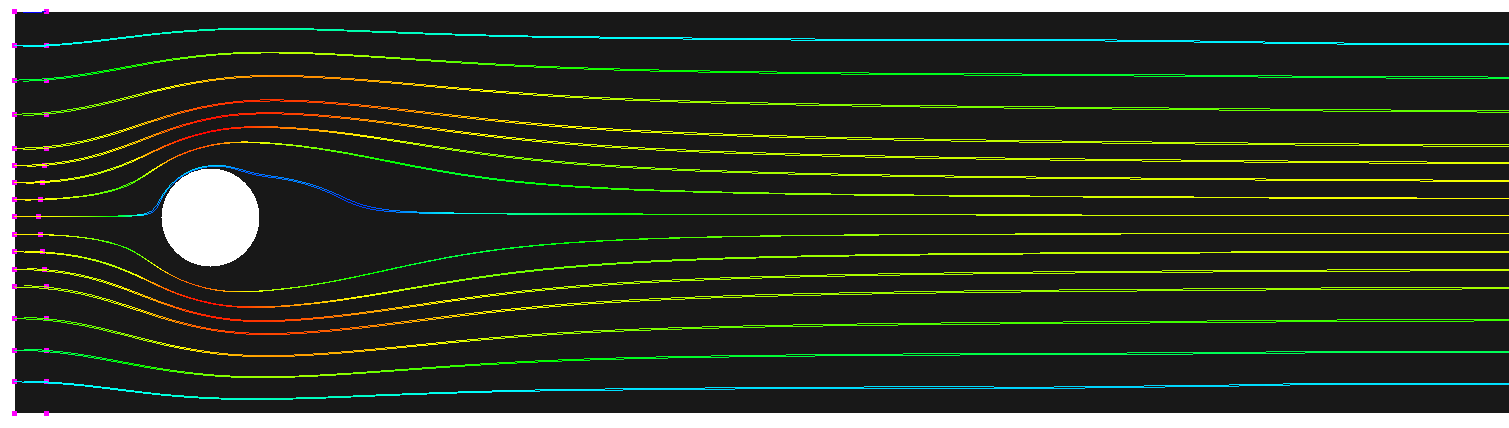
\includegraphics{screenshots/streamlines.png}};


    \end{tikzpicture}

\end{frame}

\begin{frame}

  \frametitle{Configuration of Tracer Filters}

    \begin{itemize}
      \item Tracer type filters need an \keyword{input data set} and a \keyword{seed source}
      \item The input data set is the the flow field  
      \item The seed source is a user-defined starting location for the particles inside the flow field  
    \end{itemize}
    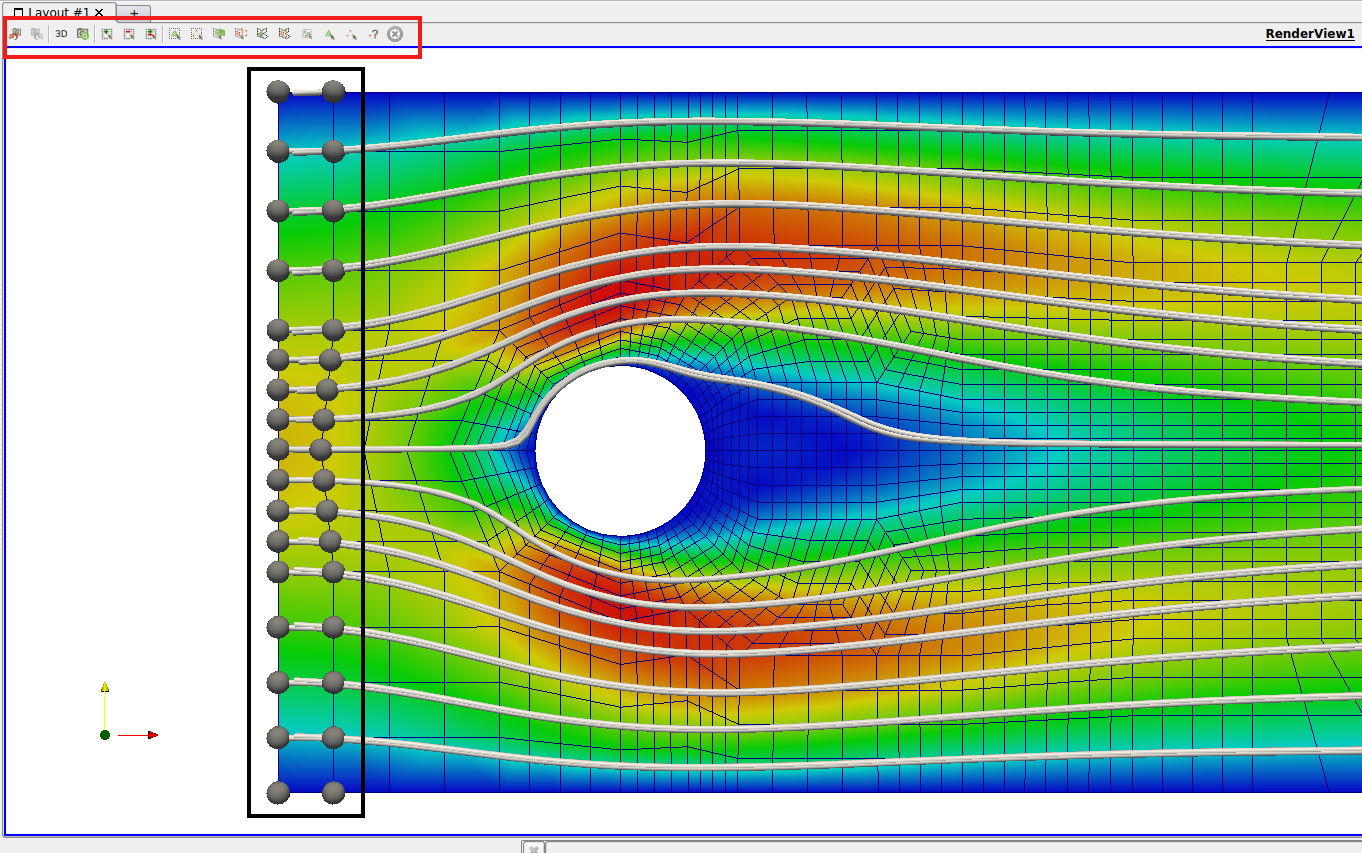
\includegraphics[width=0.5\textwidth]{screenshots/tracer-source.png}

\end{frame}

\begin{frame}

  \frametitle{Advanced Filters: Particle Tracer}

    \begin{itemize}
      \item Used to visualize transient flow data by particles 
      \item A particle path is produced by moving a particle along successive vector fields 
      \item Particle movement can then be animated by the \keyword{Animation Control} 
      \item Particle tracer example location: \kommandozeile{/mypath/to/examples/pv\_examples/AdvancedFilters/particle\_tracer}
    \end{itemize}
    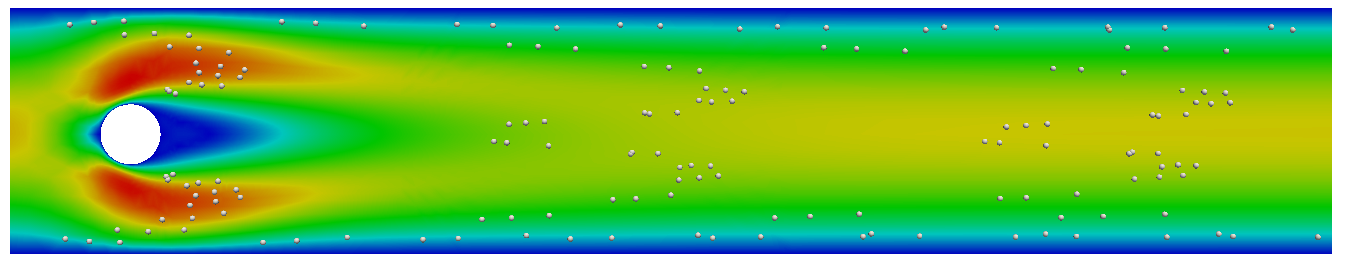
\includegraphics[width=\textwidth]{screenshots/particle-tracer.png}

\end{frame}

\begin{frame}

  \frametitle{List of Useful Filters}

    \begin{itemize}
      \item \keyword{Extract Selection}: Extract a subset from a data set (tracer source, plotting, etc)
      \item \keyword{Extract Surface}: Generates a polygonal surface mesh (exporting, rendering, remeshing) 
      \item \keyword{Clean to Grid}: Removes multiply defined simplices and converts to unstructured mesh
      \item \keyword{Integrate Variables}: Performs numerical integration of the fields defined in the data set on the mesh 
      \item \keyword{Iso-Volume or Iso-Surface}: Constructs a volume or a surface from a function defined on the mesh 
      \item \keyword{Plot Over Line}: Generates a plot of data fields along a line (inflow profiles, etc.) 
      \item \keyword{Calculator}: Use a set of mathematical operations to compute a new data field from existing ones (often used together with integrate variables filter)
    \end{itemize}

\end{frame}

\begin{frame}

  \frametitle{Input Data Formats}

    \begin{itemize}

      \item VTK data formats support polygonal data sets and structured or unstructured meshes 

      \item \keyword{VTK Legacy format .vtk} is a simple format useable for unstructured meshes (not suited for distributed data)  

      \item \keyword{VTK unstructured .vtu} is an xml based format for unstructured meshes   
    \begin{itemize}

      \item Can have the mesh data part encoded in a binary format   

      \item A \keyword{.pvtu} file can be used to reference the partial solutions of a distributed computation   

      \item A \keyword{.pvd} file can be used to add time information   

    \end{itemize}

    \item For further information on VTK file formats see:
      \url{http://www.vtk.org/VTK/img/file-formats.pdf}

  \end{itemize}

\end{frame}

\begin{frame}

  \frametitle{Scripted Postprocessing in ParaView}

  \begin{itemize}

    \item Python interface to access ParaView functionality by scripts

    \item Can be done interactively via a python shell: \keyword{Tools->Python Shell} 

    \item In a 'batch' style by passing a script to the executables \keyword{pvpython} or \keyword{pvbatch} 

    \item Documentation of the ParaView Python interface is under construction at:
      \url{https://www.paraview.org/ParaView3/Doc/Nightly/www/py-doc/}

    \item A trace mechanism is available to generate a PvPython script from a sequence of actions

    \item Beginners should use the trace mechanism (\keyword{Tools->Start Trace}) with the settings \keywords{Show Incremental Trace} and \keywords{only user-modified properties} 

    \item Upon \keyword{Tools->Stop Trace} a file is generated showing the PvPython script equivalent of the user's GUI actions
  \end{itemize}

\end{frame}

\begin{frame}

  \frametitle{PvPython Simple Example}

  \begin{itemize}
      \item PvPython simple example location: \kommandozeile{/mypath/to/examples/pv\_examples/PvPython/paraview\_python}

      \item Navigate to the folder and execute the PvPython script by: \kommandozeile{pvbatch ./python\_test.py \$(pwd)} or for versions higher than 5.1
        \kommandozeile{pvbatch {-}{-}use-offscreen-rendering ./python\_test.py \$(pwd)}

      \item The script will write an image \keyword{res.png} to the directory where you executed it 
      \item \keyword{Exercise:} Try to recreate the python script using the trace mechanism, compare the output images if they are the same.

      \item \keyword{Hint:} Prefer \keyword{pvbatch} over \keyword{pvpython} as pvpython tries to open an X windows which may fail on some computers    
  \end{itemize}

\end{frame}

\begin{frame}

  \frametitle{When to use PvPython}

  \begin{itemize}

    \item Repeated application of filters to a lot of different data sets (parameterize script w.r.t. data set) 

    \item Repeated application of operations that cannot be parametrized by ParaView GUI

    \item Perform an operation that cannot easily be done by ParaView filters 

    \item Quickly and repeatedly generate an ouput of a running simulation 

    \item Generate outputs on remote clusters 

    \item \keyword{ParaView Programmable Filter} or \keyword{Python Calculator} may serve as an alternative 

  \end{itemize}

\end{frame}

\begin{frame}

  \frametitle{Plotting with ParaView}

  \begin{itemize}

      \item PV plotting example: \kommandozeile{/mypath/to/examples/pv\_examples/Plotting/plotting.pvsm}

      \item Common ParaView plotting filters:
      \begin{itemize}

        \item \keyword{Plot Data} 

        \item \keyword{Plot Over Line} 

        \item \keyword{Plot Selection Over Time} 

      \end{itemize}

    \item Data can be exported to .csv to use in your favorite plot generator \keyword{File->Save Data}

    \item ParaView will by default export ALL data fields to the .csv file (even those that you do not want or need for the plot) 

    \item \keyword{Solution 1:} use <awk> to select the data columns you want: \kommandozeile{awk -F \textquotesingle,\textquotesingle $\;$  \textquotesingle\{print \$1 " " \$4\}\textquotesingle} (extract first and fourth column)

    \item \keyword{Solution 2:} Remove unneccessary fields before export: \kommandozeile{/mypath/to/examples/pv\_examples/Plotting/plotting2.pvsm}

  \end{itemize}

\end{frame}

\begin{frame}
  \frametitle{Client-Server Mode}

    \begin{itemize}
      \item In default mode ParaView is both the client and the server
      \item When client/server are different rendering and data processing can
        be handled by different computers 
      \item Simple X forwarding works adequately only if the network speed is fast
      \item Client-Server is preferable to access data on remote (non-local) clusters 
      \item Client-Server steps: \keyword{port forwarding}, \keyword{starting the remote server}, \keyword{connecting the client to the server}  
    \end{itemize}

    \begin{block}{Port Forwarding}
        \begin{itemize}
          \item Establish an ssh tunnel to forward the local port to the remote server: \\  
          \kommandozeile{> ssh lidong1.itmc.tu-dortmund.de \textbackslash}
          \kommandozeile{-L 11111:lidong1.itmc.tu-dortmund.de:11111}
        \end{itemize}
    \end{block}

\end{frame}

\begin{frame}
  %\frametitle{Client-Server Mode II}

    \begin{block}{Start the remote Server}
        \begin{itemize}
          \item Start a ParaView data server on the remote machine  
            \kommandozeile{> pvserver {-}{-}server-port=11111 {-}{-}use-offscreen-rendering}
        \end{itemize}
    \end{block}

    \begin{block}{Connect to the remote Server}
        \begin{itemize}
          \item Start a ParaView client locally  
          \item Press the <Connect> button on the toolbar  
          \item Manually configure the Server dialog:
          \begin{itemize}
            \item Name: myname   
            \item Server Type: Client/Server  
            \item Host: localhost 
            \item Port: 11111 
          \end{itemize}
        \end{itemize}
    \end{block}
  Pitfalls:
    \begin{itemize}
      \item You \textbf{have to} make use the same ParaView version of the client and the server
      \item Check that the port is not occupied, otherwise use a different port: 
      \kommandozeile{> lsof -i:11111}
    \end{itemize}

\end{frame}

\begin{frame}

  \frametitle{Additional ParaView Resources}

  \begin{itemize}
      \item ParaView documentation:\\
        \url{https://www.paraview.org/documentation/}
      \item ParaView Wiki:\\
        \url{https://www.paraview.org/Wiki/ParaView}
      \item ParaView Tutorial:\\
        \url{https://www.paraview.org/Wiki/The\_ParaView\_Tutorial}
      \item ParaView Mailing List:\\
        \url{https://public.kitware.com/mailman/listinfo/paraview}
      \item ParaView Catalyst:\\
        \url{https://www.paraview.org/Wiki/ParaView/Catalyst/Overview}
      \item ParaView Web JavaScript:\\
        \url{www.paraview.org/Wiki/ParaViewWeb\_JavaScript\_Introduction}
  \end{itemize}

\end{frame}

